\section{Average Relative Error}
\label{section:results_are}

\subsection*{Purpose}

\paragraph{}
To compare the average relative error of each sketch under different types of graph streams.

\paragraph{}
Average relative error has been previously defined in \autoref{section:metrics_are}. For this section of testing, the average relative error of simple edge frequency queries has been measured.

\subsection*{Results}

\begin{figure}[H]
    \centering 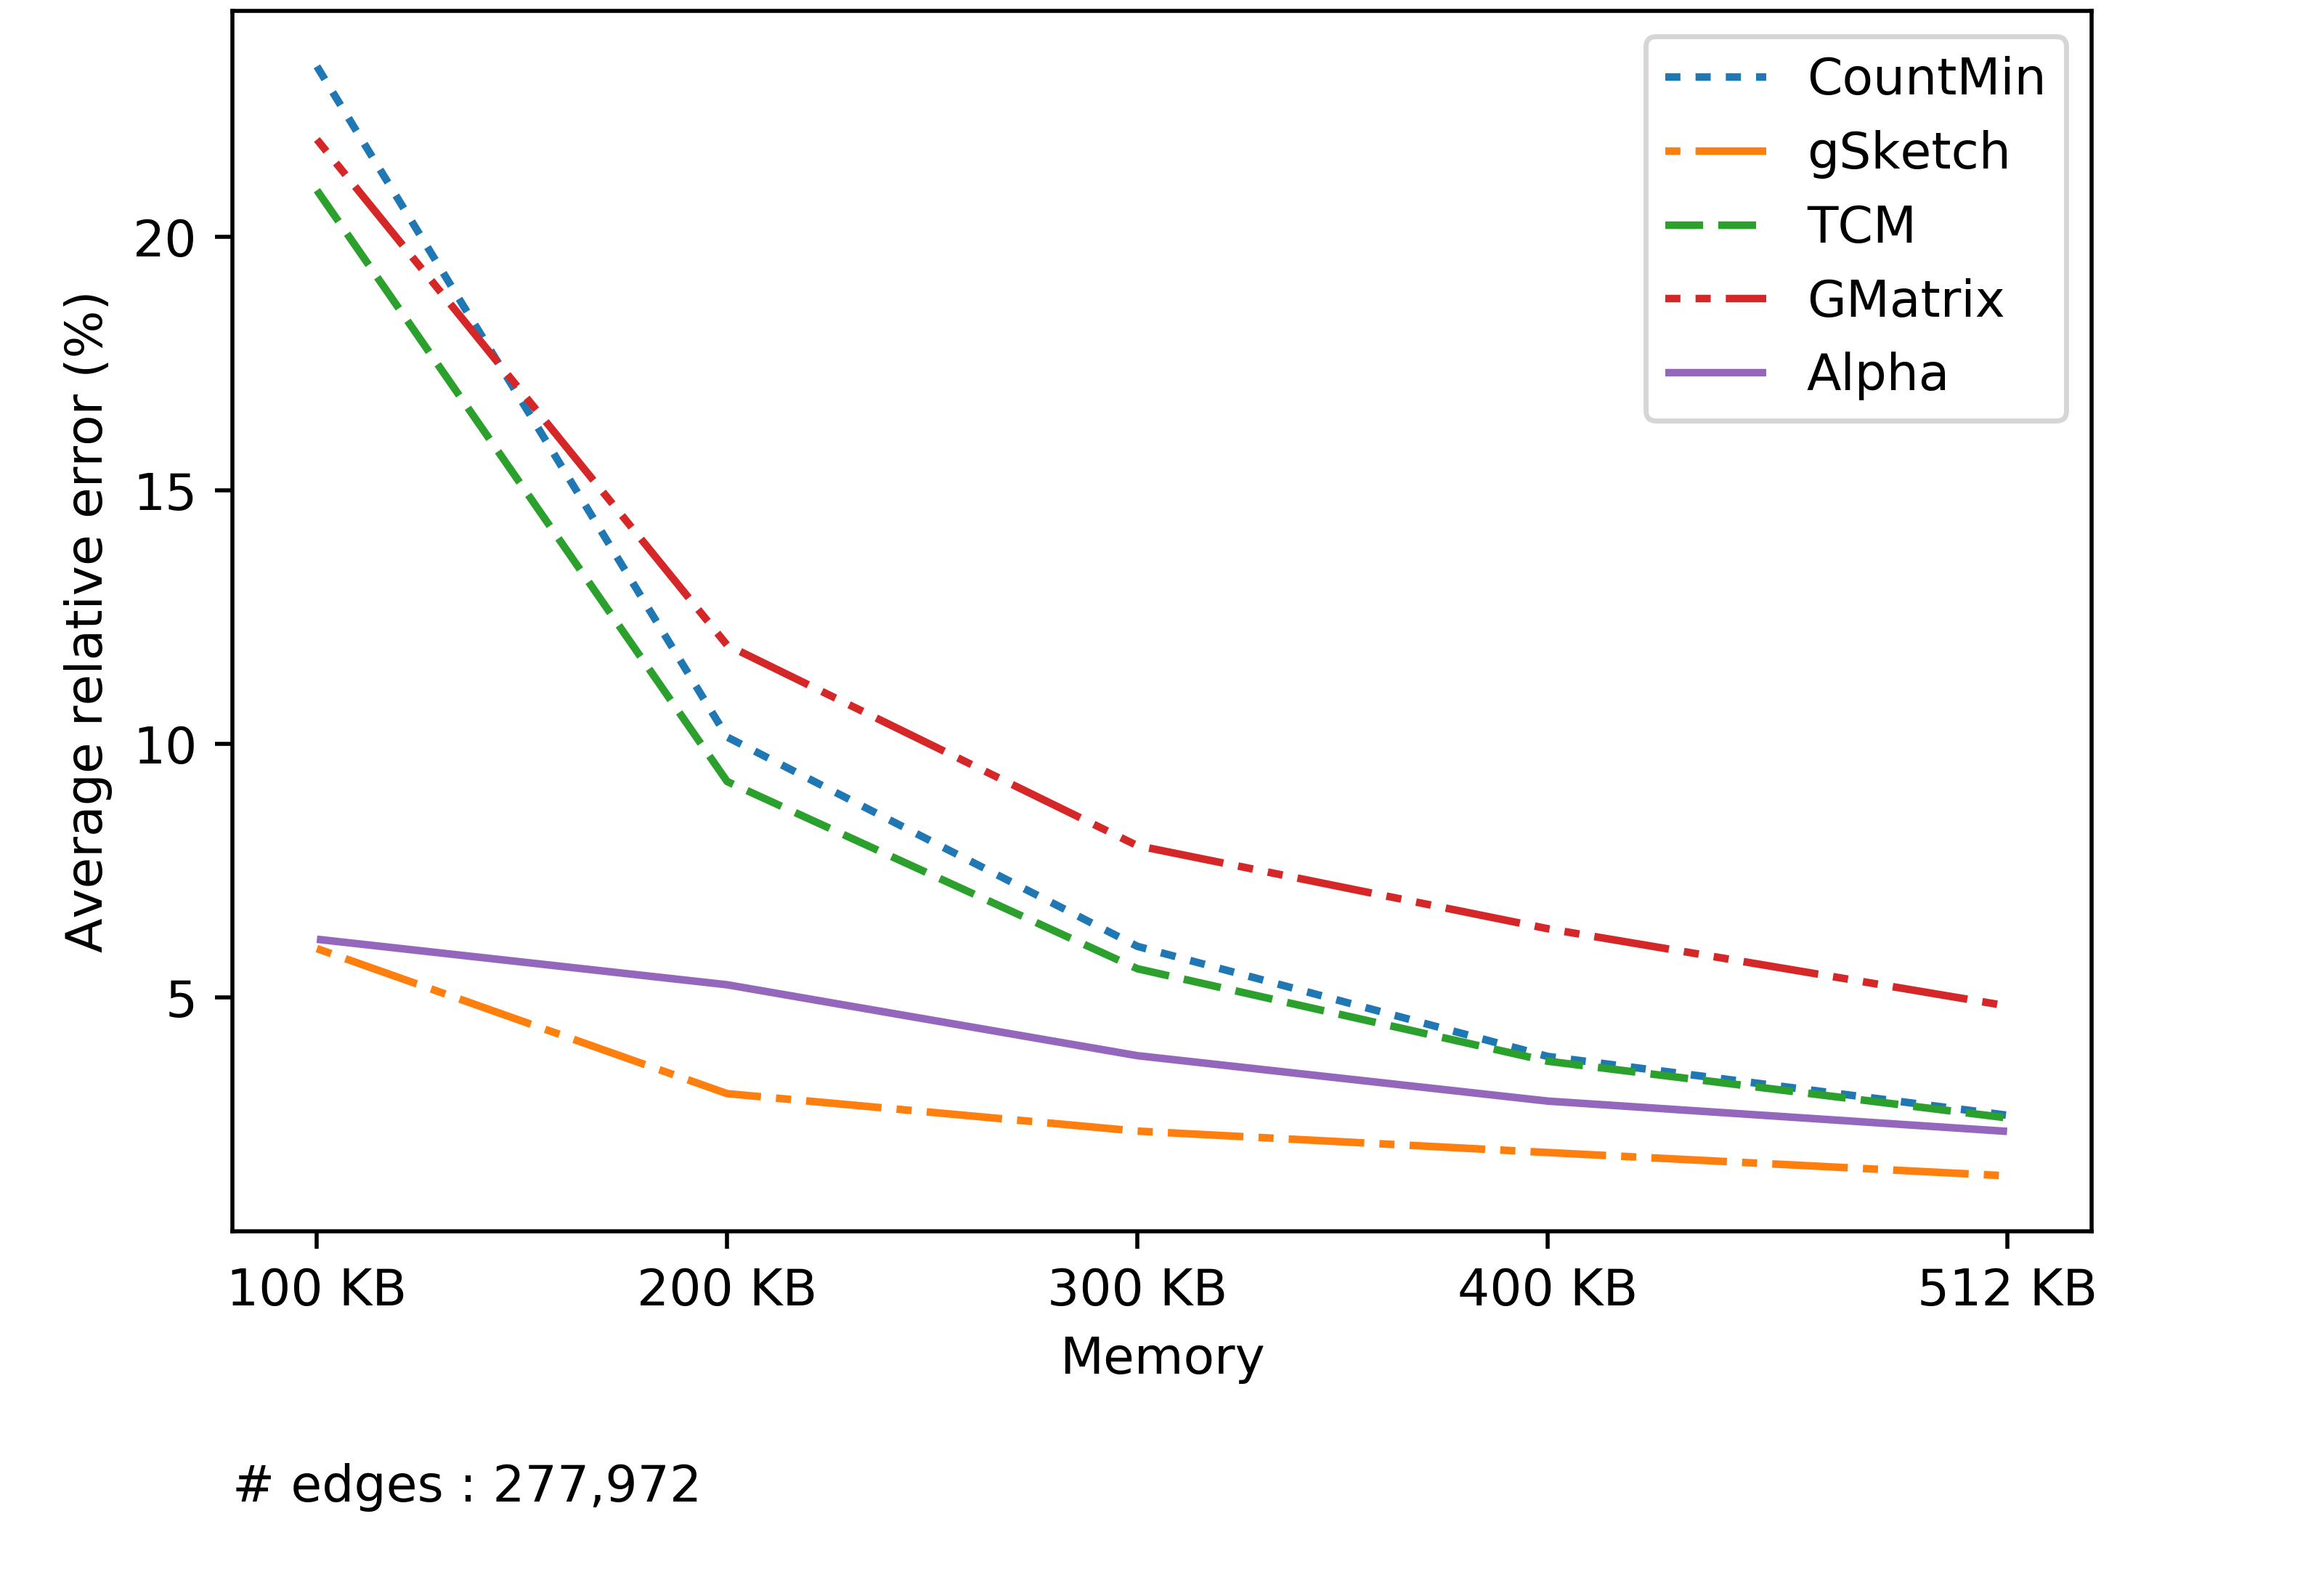
\includegraphics[width=0.85\textwidth]{results/are/unicorn-wget-are}
    \vspace{-0.5cm}
    \caption{Average relative error vs Memory for unicorn-wget dataset}
    \label{fig:unicorn-wget-are}
\end{figure}

\begin{figure}[H]
    \centering 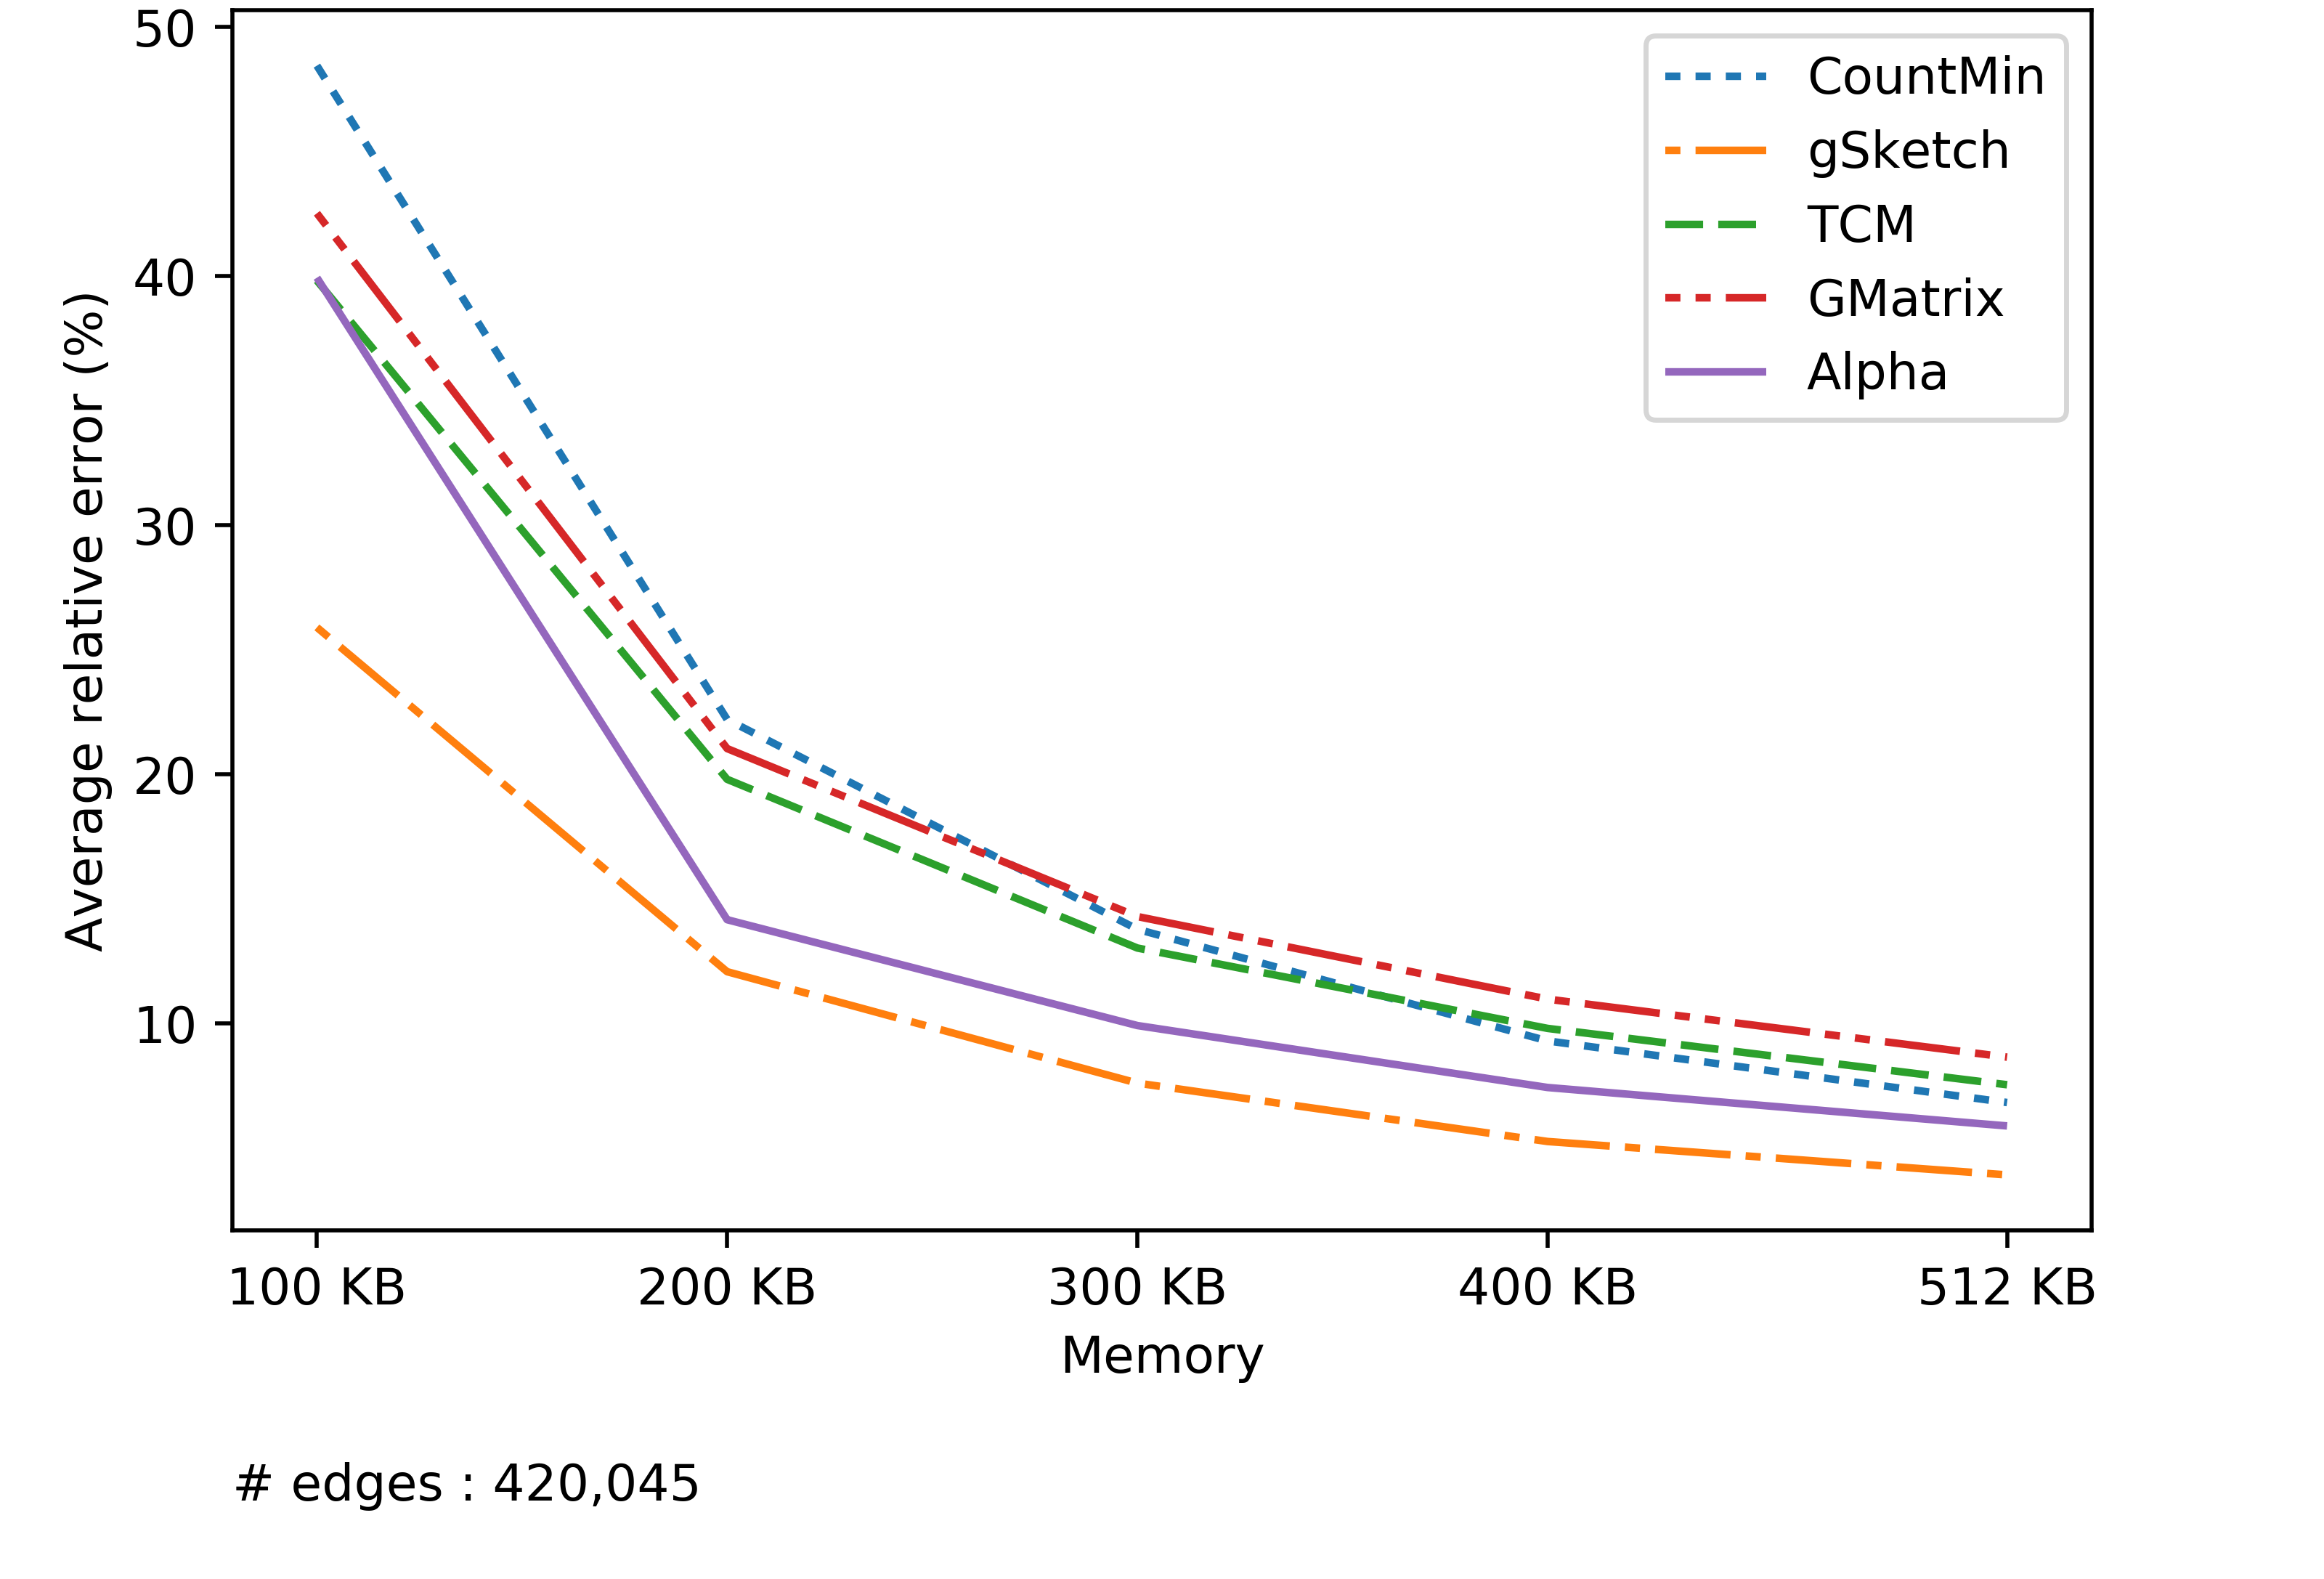
\includegraphics[width=0.85\textwidth]{results/are/email-EuAll-are}
    \vspace{-0.5cm}
    \caption{Average relative error vs Memory for email-EuAll dataset}
    \label{fig:email-EuAll-are}
\end{figure}

\begin{figure}[H]
    \centering 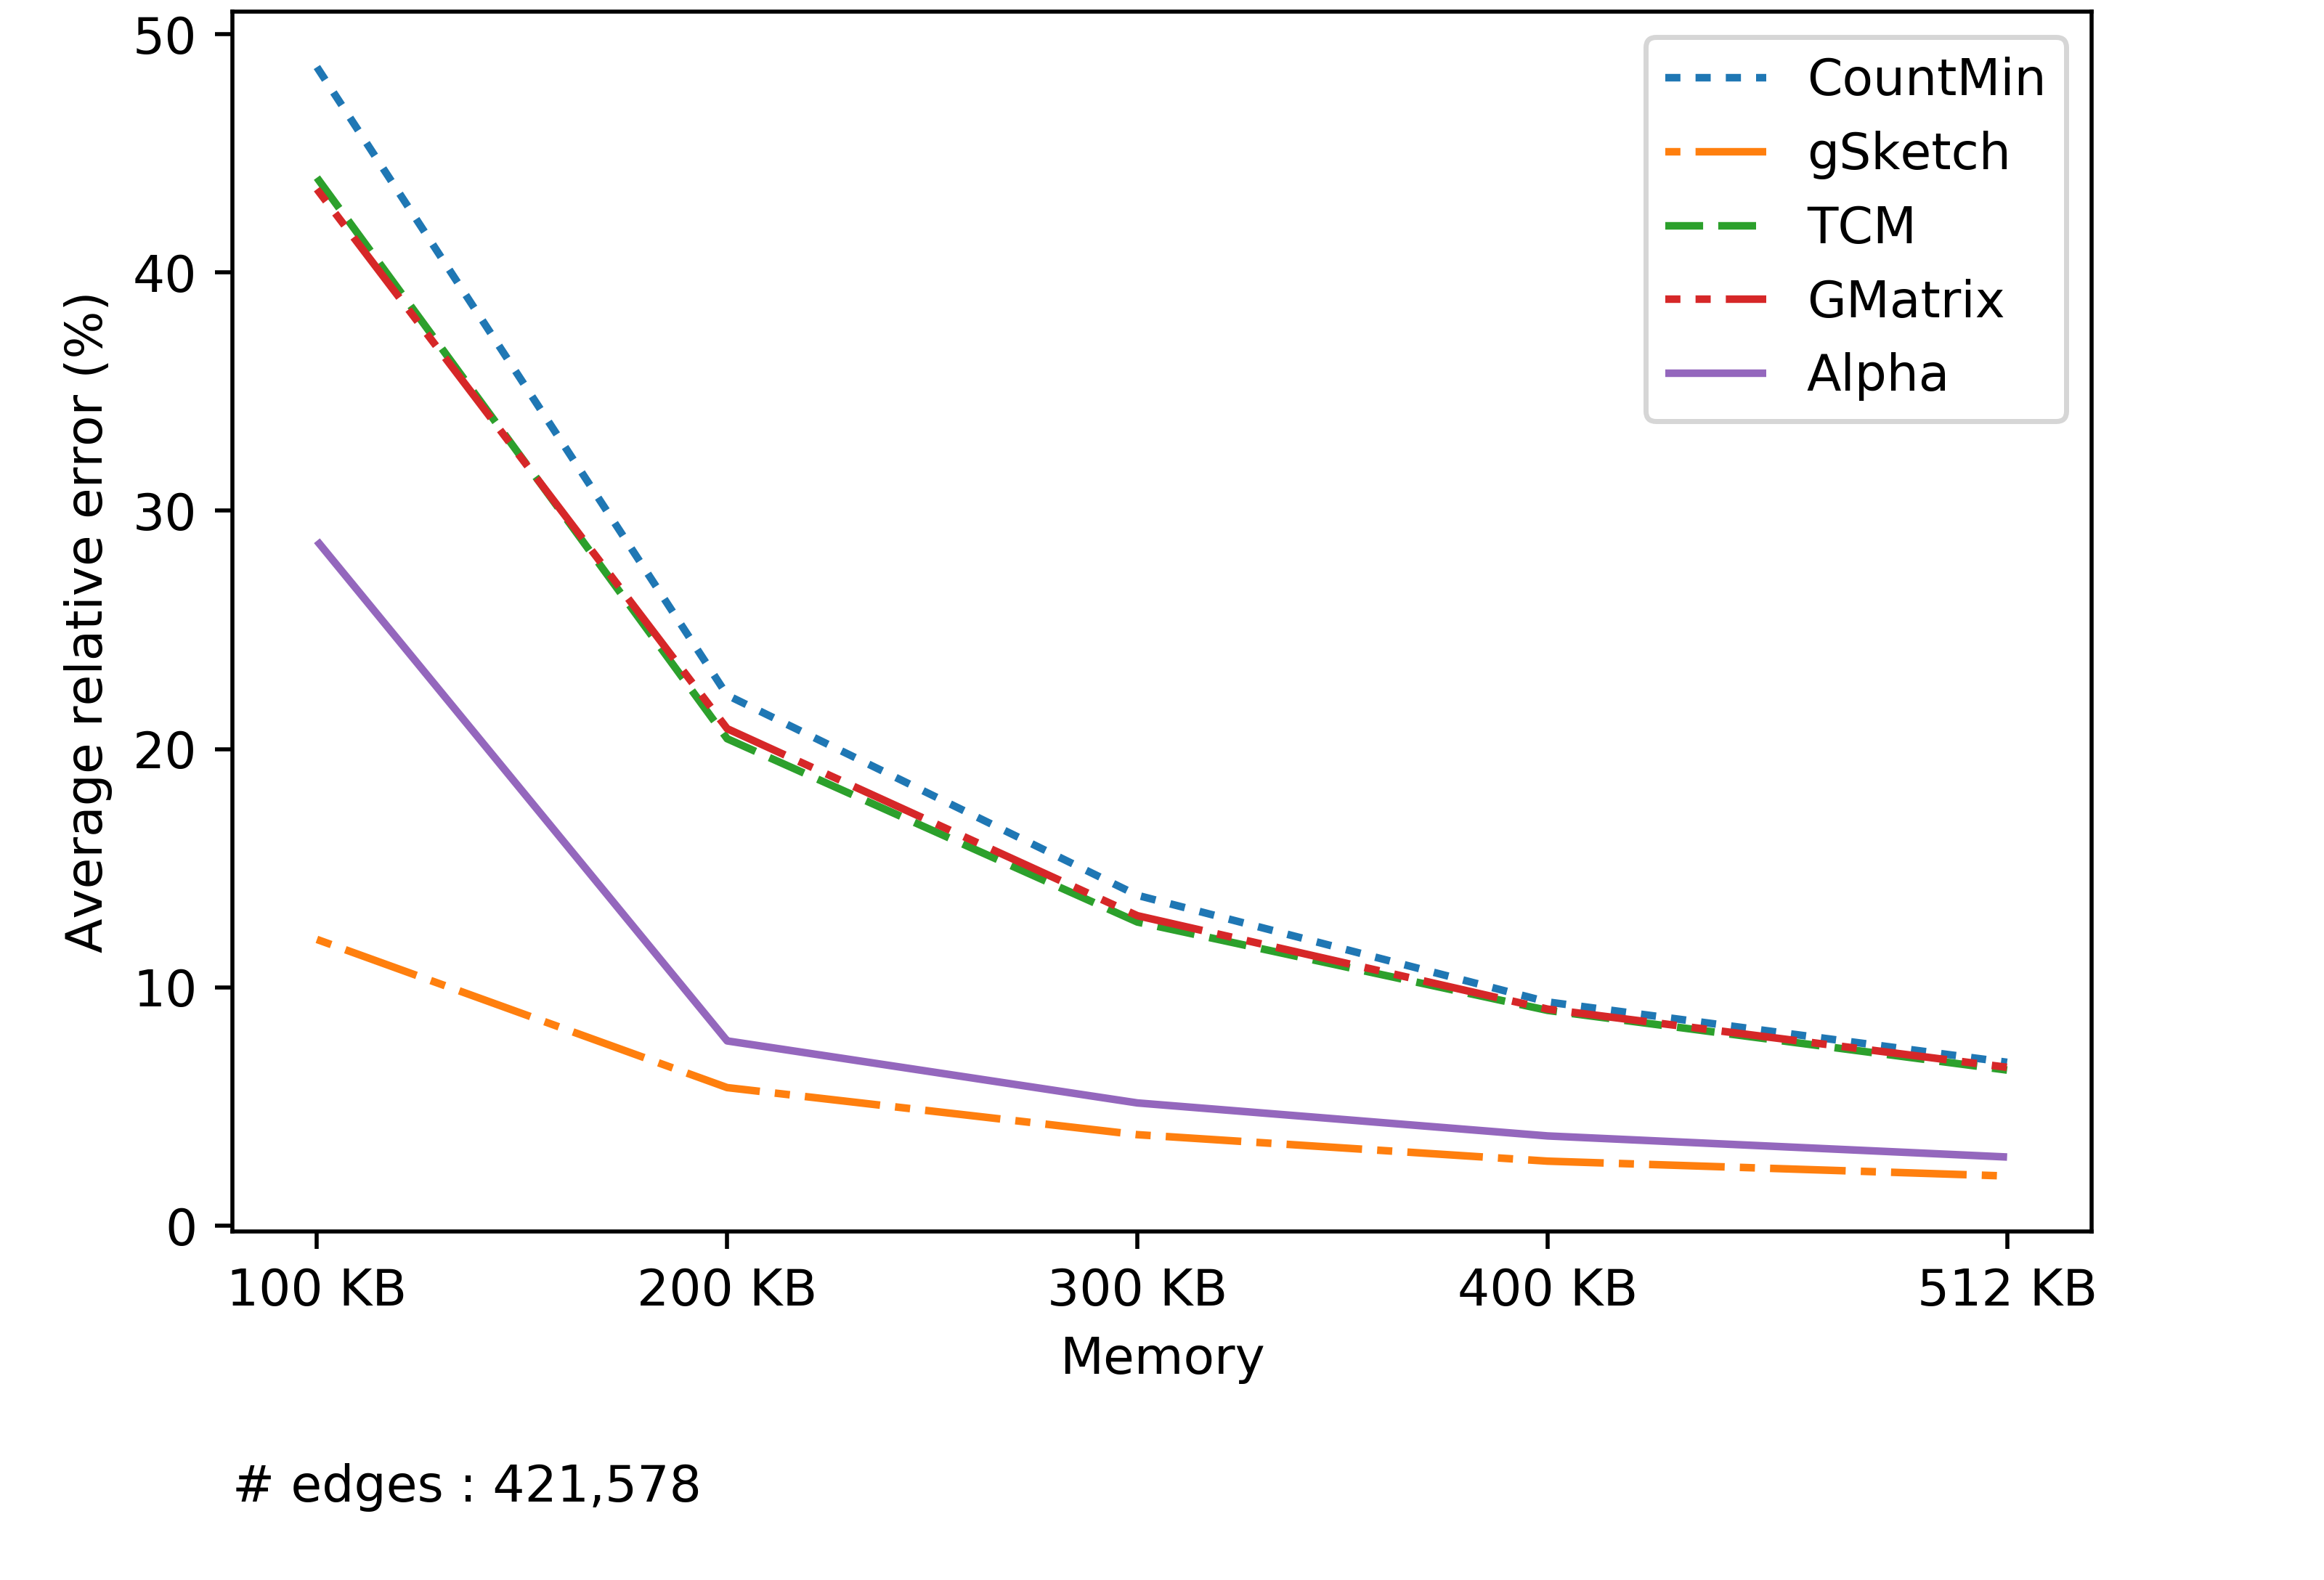
\includegraphics[width=0.85\textwidth]{results/are/cit-HepPh-are}
    \vspace{-0.5cm}
    \caption{Average relative error vs Memory for cit-HepPh dataset}
    \label{fig:cit-HepPh-are}
\end{figure}

\begin{figure}[H]
    \centering 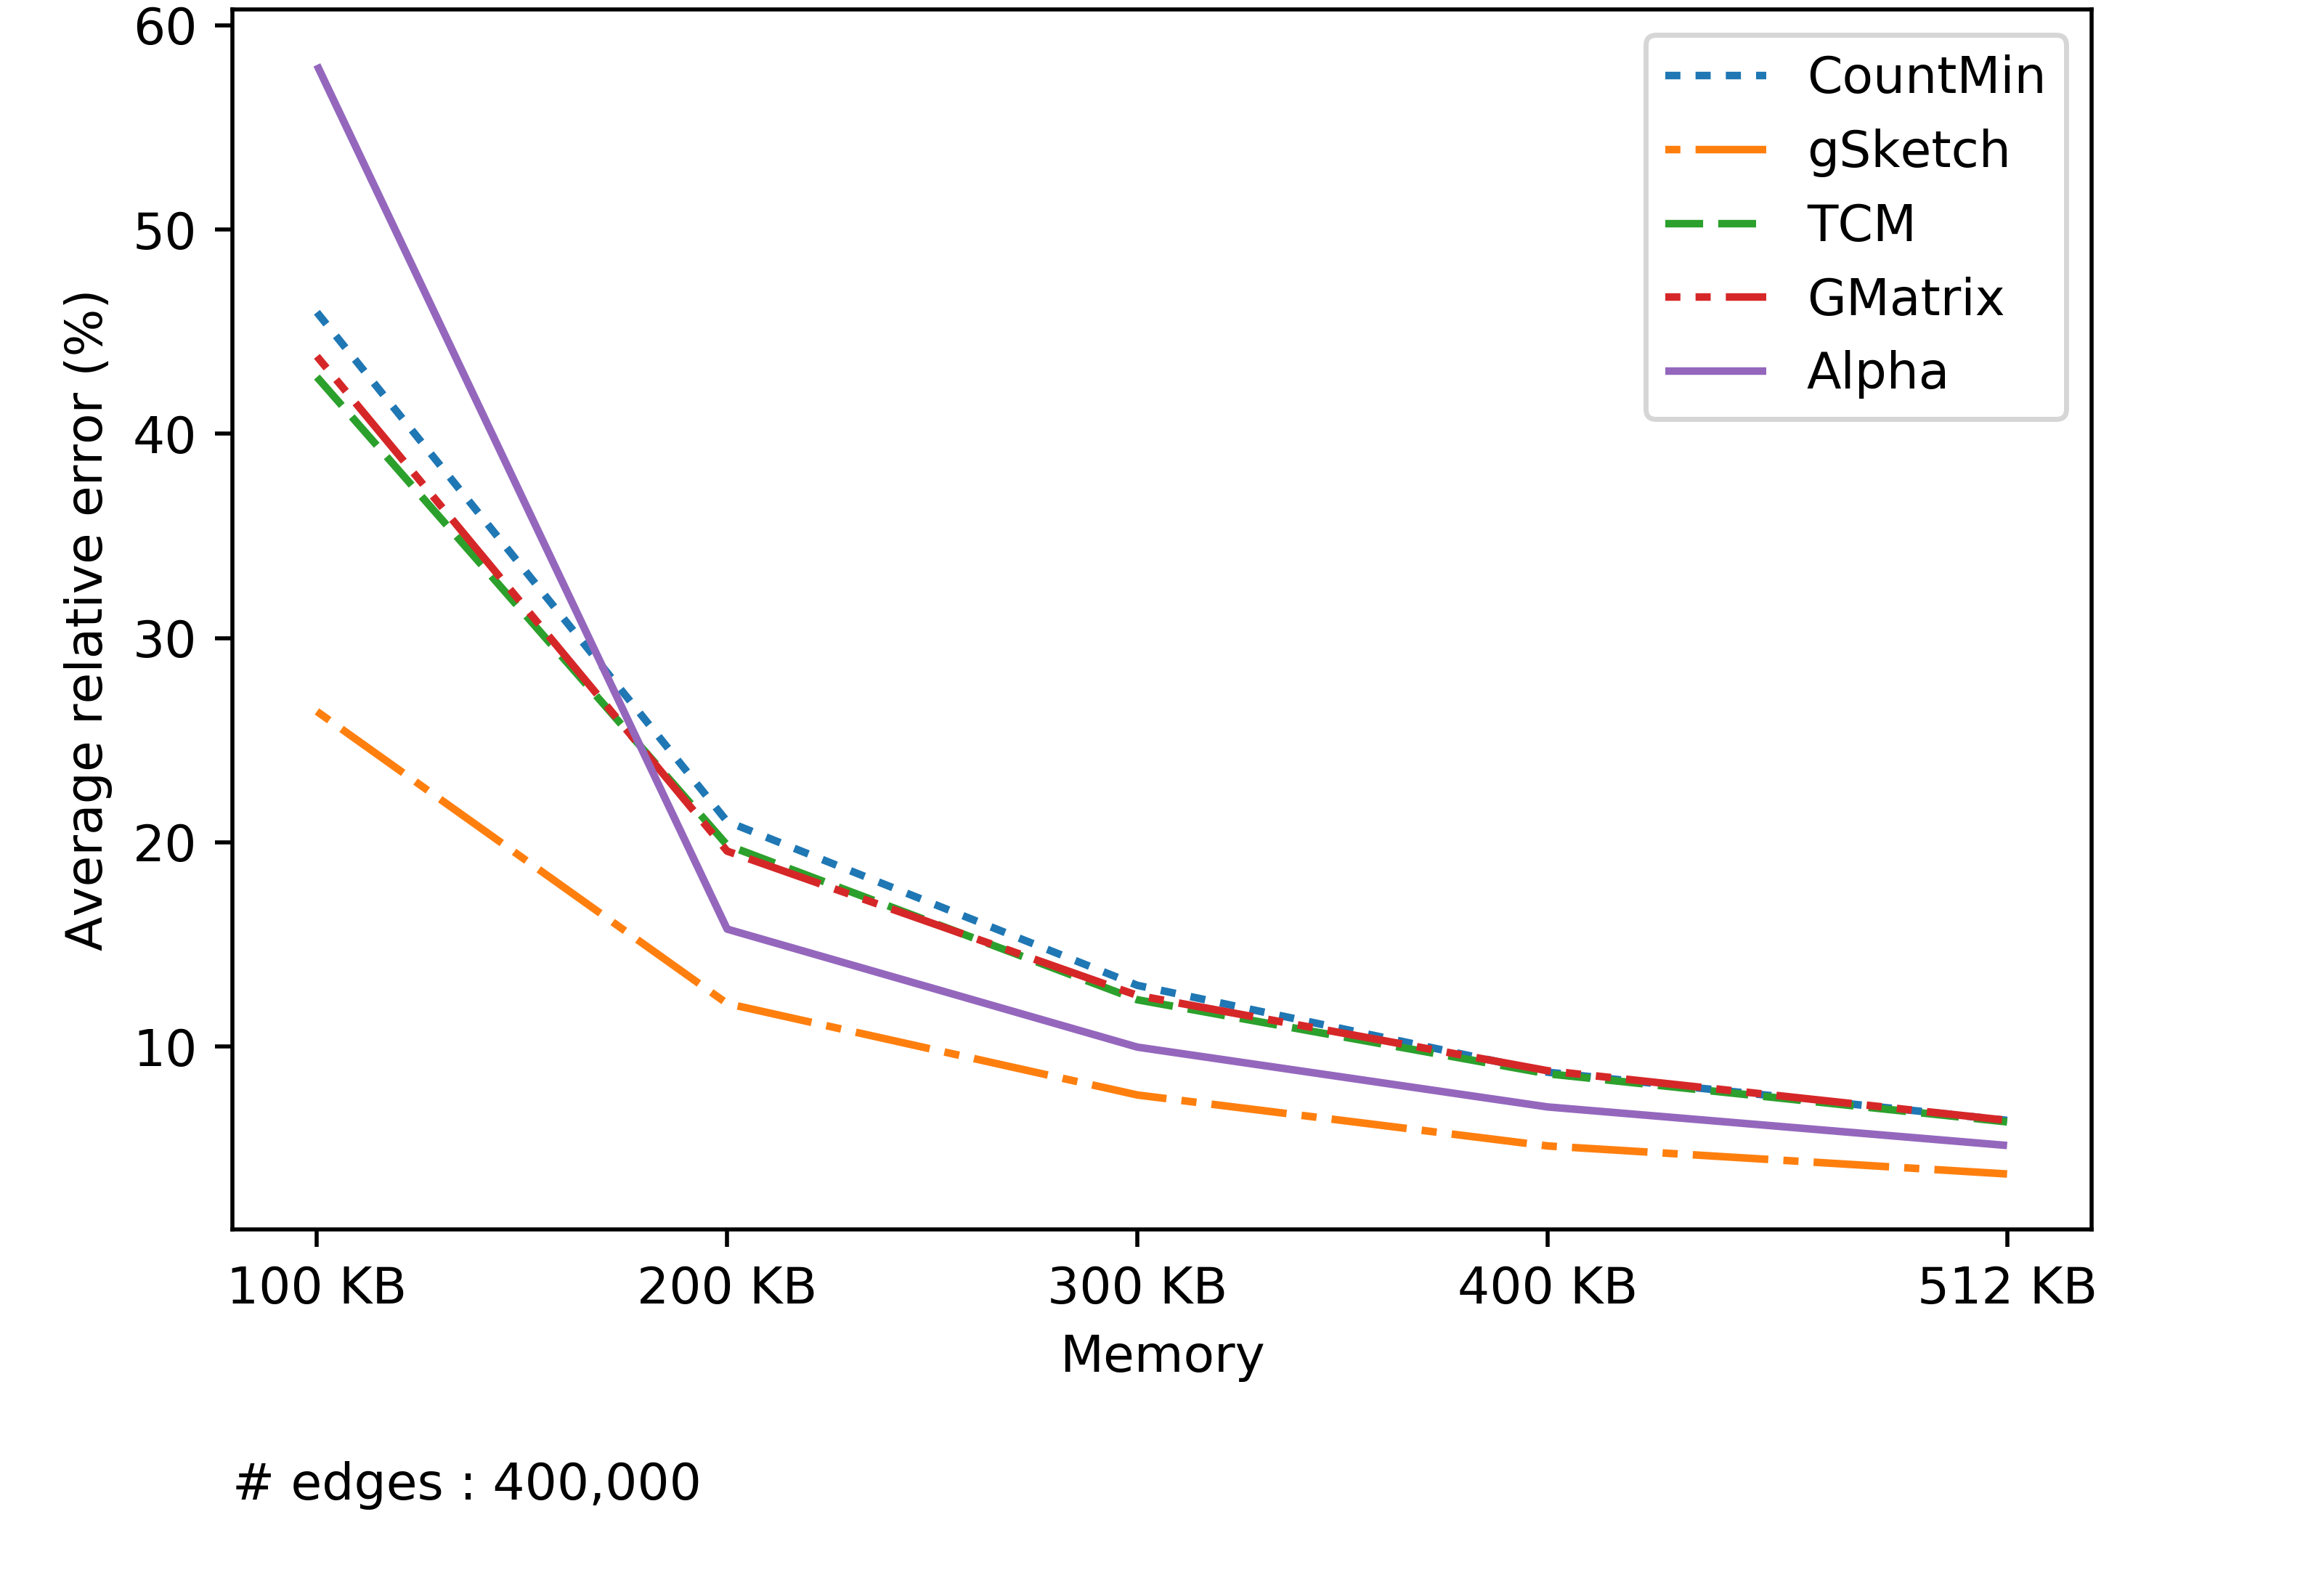
\includegraphics[width=0.85\textwidth]{results/are/gen-scale-free-are}
    \vspace{-0.5cm}
    \caption{Average relative error vs Memory for gen-scale-free dataset}
    \label{fig:gen-scale-free-are}
\end{figure}

\begin{figure}[H]
    \centering 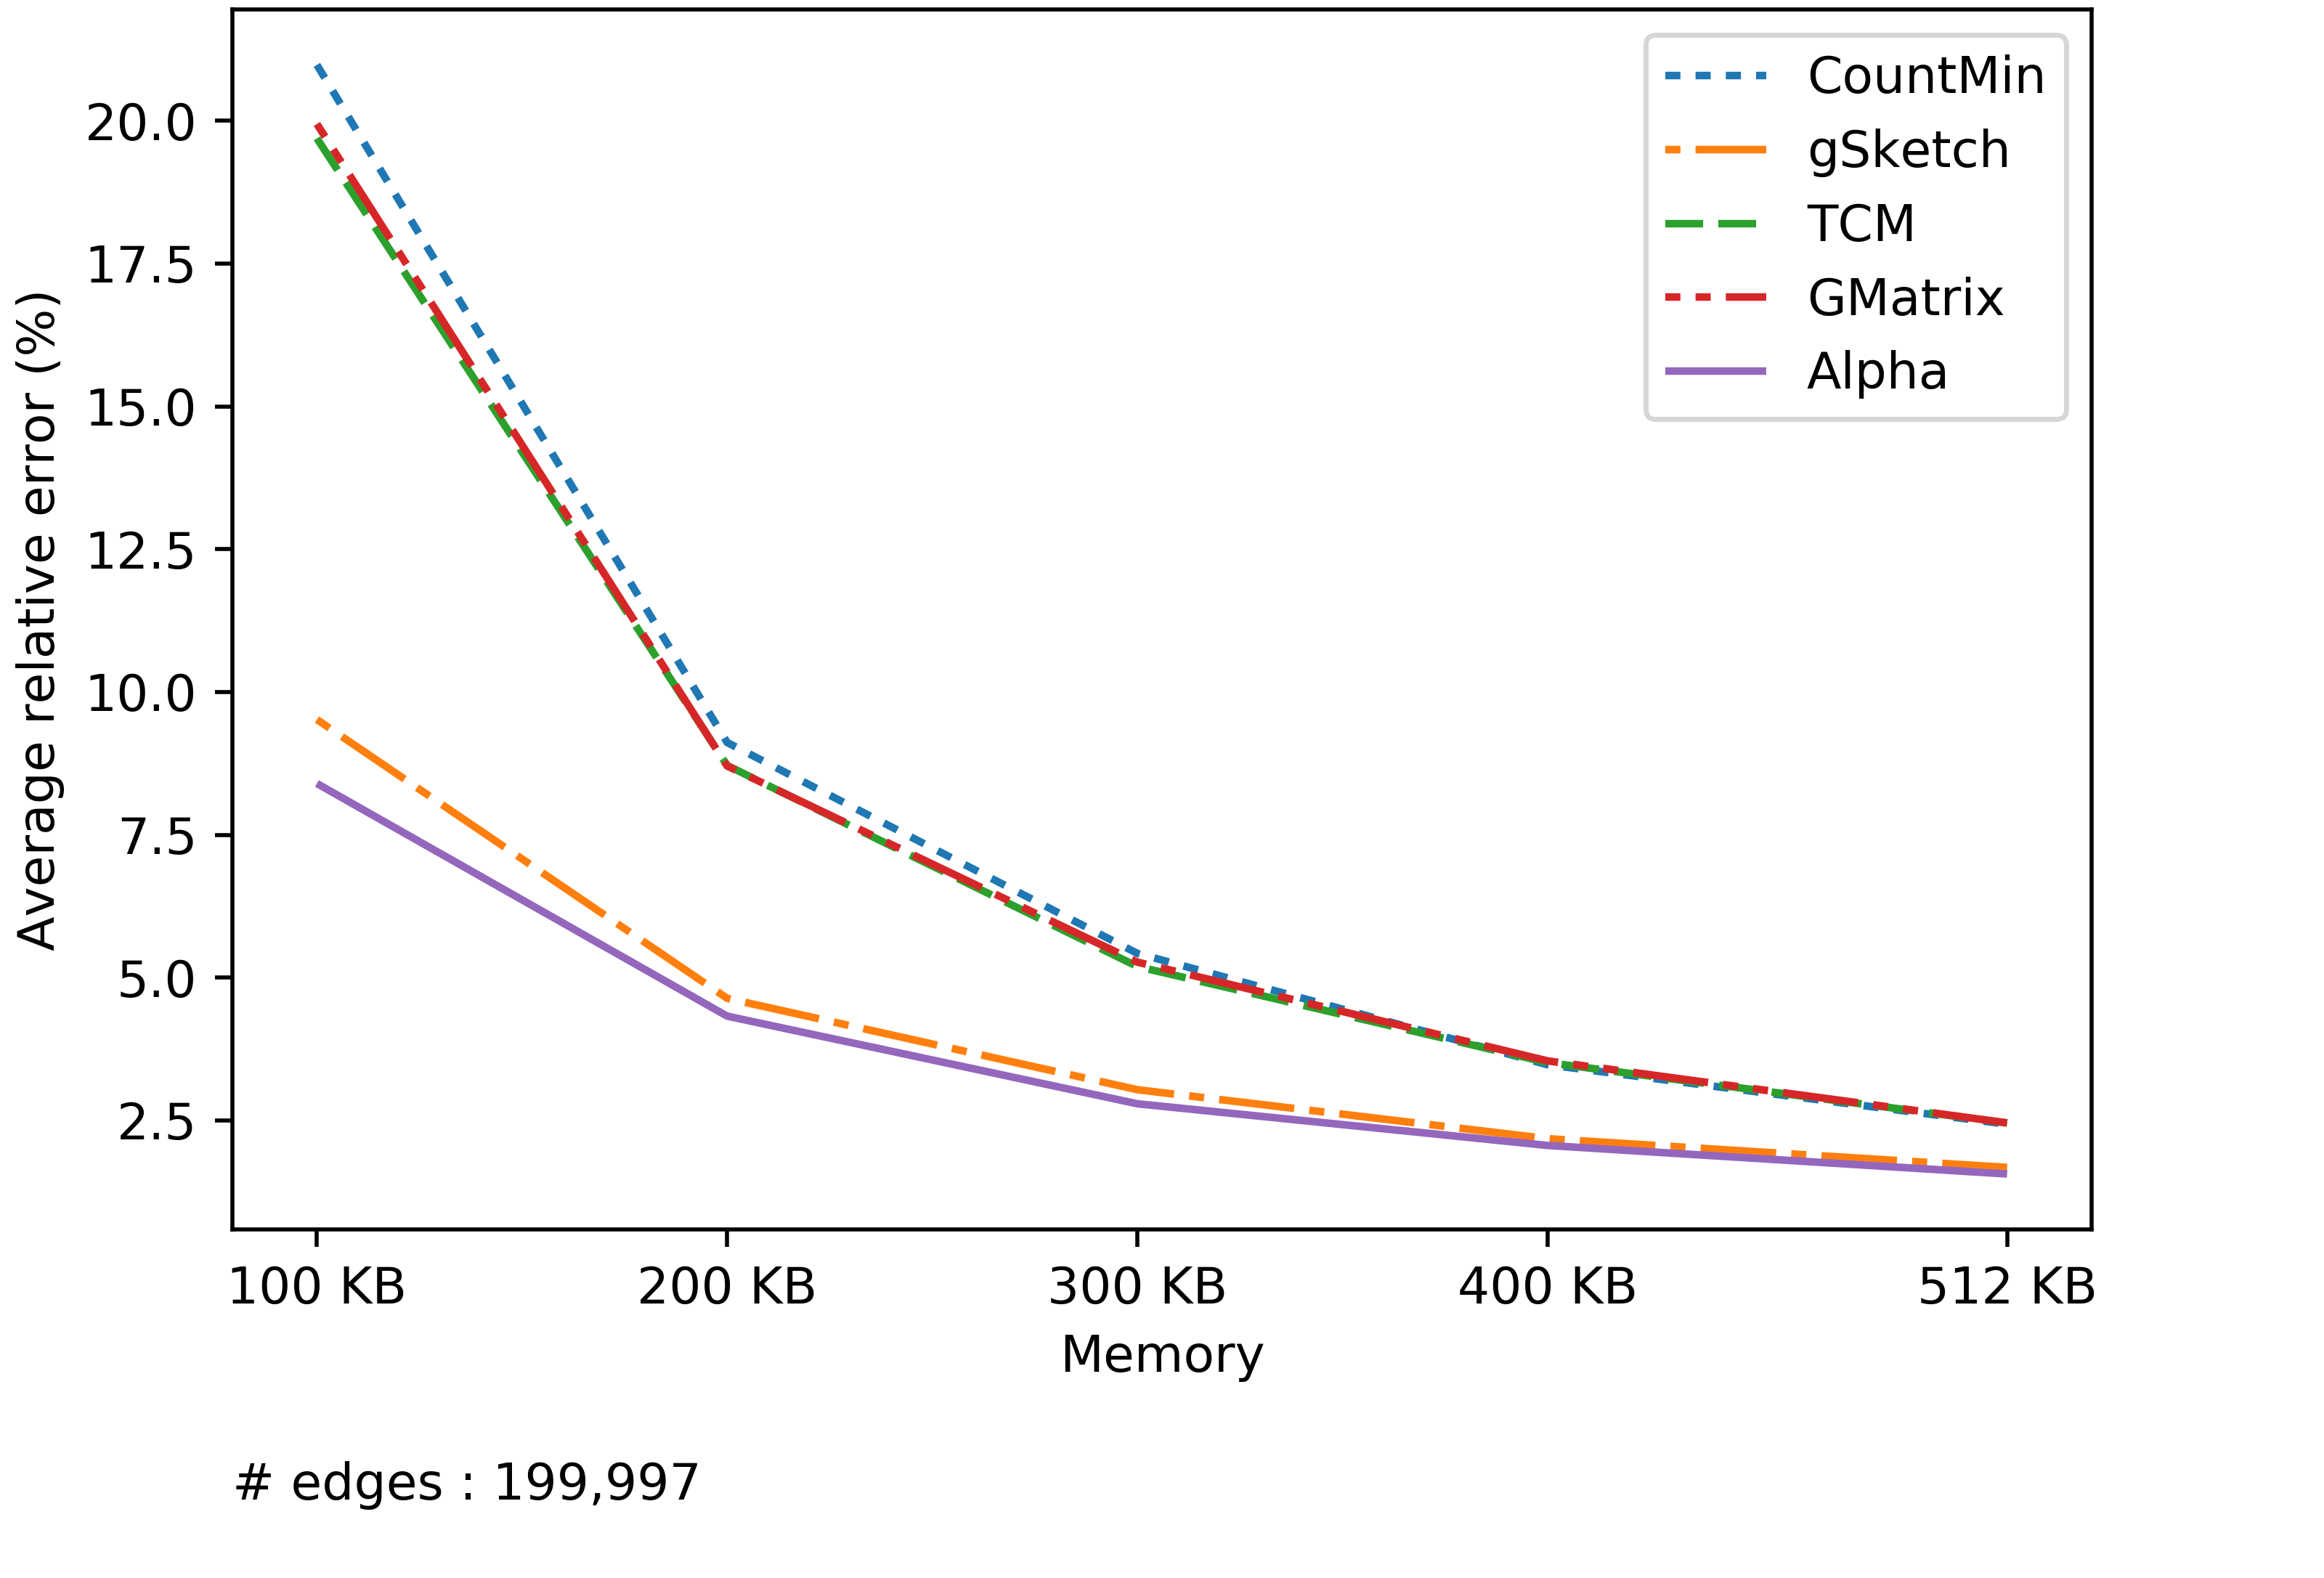
\includegraphics[width=0.85\textwidth]{results/are/gen-small-world-are}
    \vspace{-0.5cm}
    \caption{Average relative error vs Memory for gen-small-world dataset}
    \label{fig:gen-small-world-are}
\end{figure}

\subsection*{Observations and inferences}

\paragraph{}
In the results for the datasets, unicorn-wget in \autoref{fig:unicorn-wget-are}, email-EuAll in \autoref{fig:email-EuAll-are}, cit-HepPh in \autoref{fig:cit-HepPh-are}, gen-scale-free in \autoref{fig:gen-scale-free-are} and gen-small-world in \autoref{fig:gen-small-world-are}; Alpha has a significantly lower average relative error in general than all the other sketches except for gSketch.

\paragraph{}
In the \autoref{fig:gen-scale-free-are}, for 100 KB sketch size, Alpha has a higher average relative error than all the other sketches. This could possibly be a result of over-partitioning a smaller sketch such that the final error of the queries are worse than the unpartitioned sketch.

\paragraph{}
Alpha has the lowest average relative error for the gen-small-world dataset depicted in \autoref{fig:gen-small-world-are}. Thus it is evidant that Alpha is able to surpass the accuracy levels of gSketch in some cases.

\paragraph{}
Alpha has a much lower average relative error than TCM and GMatrix for all the tested datasets, proving its superiority over the existing sketching algorithms. It has even surpassed approximate frequency sketches like CountMin in this regard.